%%%%%%%%%%%%%%%%%%%%%%%%%%%%%%%%%%%%%%%%%%%%%%%%%%%%%%%%%%%%%%%%%%%%%%%%%%%%
%% Thesis Template - Tilburg Science Hub
%% Andrea Domenico Antonacci, a.d.antonacci@tilburguniversity.edu
%% Last update: April 2021
%% Use pdflatex
%%%%%%%%%%%%%%%%%%%%%%%%%%%%%%%%%%%%%%%%%%%%%%%%%%%%%%%%%%%%%%%%%%%%%%%%%%%%

%% INSTRUCTIONS:
%% Use this file to define the document structure, the preamble, the abstract, and the acknowledgements.
%% Use the section files to write your content and import them here.
%% This template is meant to run on pdflatex and with fonts available via packages.
%% Use XeLaTeX if you want to use your own custom fonts.

\RequirePackage{amsmath} % Load amsmath first
\documentclass[a4paper,12pt]{article}
% Set your margins here
\usepackage[margin=1in]{geometry}
% Set your language
\usepackage[english]{babel}
\usepackage[utf8]{inputenc}
% Define fonts via packages
\usepackage{mathpazo} % Use Palatino font
% \usepackage{gfsdidot} % Or use Didot font
% Set global line spacing
\renewcommand{\baselinestretch}{1.5}
% Allow multi-column environments
\usepackage{multicol}
\setlength\columnsep{40pt}
% Formulas and math
\usepackage{amssymb}
\usepackage{mathtools}
\usepackage{empheq}
\usepackage{units} % Allow nice in-line, diagonal fractions
% Define bibliography, update according to your needs
\usepackage[
    backend=biber,
    style=numeric,
  ]{biblatex}
 \addbibresource{bib.bib}
% Allow hyperref with click-through sections and references
\usepackage[unicode=true,pdfusetitle,bookmarks=true,bookmarksnumbered=true,bookmarksopen=true,bookmarksopenlevel=1,breaklinks=false,pdfborder={0 0 0},pdfborderstyle={},backref=false]{hyperref}
% Replace "Placeholder Name" in pdfauthor with your real name and update the link colors to taste
\hypersetup{pdfpagelayout=OneColumn, pdfnewwindow=true, pdfstartview=XYZ, plainpages=false,pdfauthor={Placeholder Name},colorlinks=true,linkcolor=ForestGreen,citecolor=ForestGreen}
% Allow fancy headers
\usepackage{fancyhdr}
\fancypagestyle{SectionFirstPage}{\fancyhead{}\renewcommand{\headrulewidth}{0pt}} % Use this pagestyle to hide headers on the first page of sections
% Misc packages
\usepackage{lipsum} % For prototyping
\usepackage{listings} % To highlight code
\usepackage{algorithm} % For algorithms
\usepackage{setspace} % To set line spacing locally
\usepackage{graphicx} % Allow figures
\graphicspath{ {images/} } % Specify the path for images
\usepackage[dvipsnames]{xcolor} % Enable more colors in text
\usepackage{microtype} % Improve justification
\usepackage{url} % Line-breaking urls
\usepackage{pdflscape} % Allow pages in landscape mode
\usepackage{multirow} % Allow multirow in tables
\usepackage[labelfont=bf]{caption} % Set caption distances from tables and figures
\usepackage{subcaption} % For subfigures, remove if unused
\captionsetup[table]{skip=10pt, position=top}
\captionsetup[figure]{belowskip=10pt, skip=5pt, position=top}
\usepackage[nottoc]{tocbibind} % Add bibliography to Table of Content
\usepackage{makecell} % Allow to break lines inside a table cell
\usepackage[para]{threeparttable} % For structured and complex tables
\usepackage{rotating} % To rotate tables
\usepackage{textcomp} % For symbols
\usepackage{tikz} % For graphs and graphics
\usetikzlibrary{shapes.geometric, shapes.misc, arrows, positioning}
\def\checkmark{\tikz\fill[scale=0.4](0,.35) -- (.25,0) -- (1,.7) -- (.25,.15) -- cycle;} % Define a checkmark (tick), used in section 2
\usepackage{varioref} % Intelligent references with pageref automatically added
\setlength{\headheight}{14.49998pt}
\counterwithin*{equation}{section} % Reset numbering for each chapter
\counterwithin*{equation}{subsection}
\newenvironment{system}%
{\left\lbrace\begin{array}{@{}l@{}}}%
{\end{array}\right.}
% Define title page
\usepackage{titling}
\renewcommand\maketitlehooka{\null\mbox{}\vfill} % To vertically center it
\renewcommand\maketitlehookd{\vfill\null}
\title{ 
    Mathematical Theory of Infectious Disease Epidemics \\
        \large Final Project in Numerical Methods \\ American University of Armenia \\
}
\author{Grigor Hovhannisyan
\and
Aram Abrahamyan
\and
Meruzhan Khachatryan
}
% \date{January 2000} % Uncomment for custom date

%%%%%%%%%%%%%%%%%%%%%%%%%%%%%%%%%%%%%%%%%%%%%%%%%%%%%%%%%%%%%%%%%%%%%%%%%%%%
%% CONTENT BELOW
%%%%%%%%%%%%%%%%%%%%%%%%%%%%%%%%%%%%%%%%%%%%%%%%%%%%%%%%%%%%%%%%%%%%%%%%%%%%

\begin{document}



% Title page
{ % Use curly brackets to create a group and assign properties locally
\setstretch{1.0}
\maketitle\thispagestyle{empty}
\vspace{1cm}{}
}
\vspace{1cm}


% Table of Content
{
    \newpage
    \setstretch{1.0}
    \hypersetup{linkcolor=black} % Links in TOC are black
    \pagenumbering{roman}
    \tableofcontents
    \listoffigures
}

% Abstract
\newpage
\begin{abstract}
    \addcontentsline{toc}{section}{Abstract}
    Infectious diseases are a prevalent issue among everyone.
    The knowledge of its likely path and development can substantially help the government control the disease and hospitals correctly manage resources to accommodate the high number of patients.
    This is the aim of the SIR model, which this paper aims to explain and provide examples of.
    The SIR model has many modifications and extensions, some of which we will explore.
    We will also showcase and explain the analytic solution to the standard SIR model, but unfortunately, many of the modifications do not have an analytical solution; hence, we will approximate them numerically.
    The main methods to do so will be the Euler and the backward Euler methods, both of which have an error, which we will derive and showcase on graphs.
    All of the coding is done in Python with examples and explanations, as well as graphs and the explanation of the given graphs.
    Furthermore, we gathered and plotted graphs from real-world data concerning some famous diseases.
    We will compare them to the SIR model and determine how accurate it gets over time.
    Finally, we will draw conclusions and discuss how much of an impact the model can have on the world if used correctly.
\end{abstract}

% Content
\newpage
\pagestyle{fancy} % Initiate headers
% Define global headers for all the sections
\lhead{\nouppercase{\rightmark}}
\rhead{}
\pagenumbering{arabic}
% Import sections
\section{Introduction}\label{Introduction}\thispagestyle{SectionFirstPage} % Hide headers on the first page of the section
\lhead{Introduction to Epidemic Modeling}
\hspace{\parindent} Infectious disease epidemics cause significant challenges to public health, necessitating mathematical models for understanding and managing their spread.
The practical use of epidemic models must rely heavily on the realism put into the models.
This means that a reasonable model can include only some possible effects but rather incorporate the mechanisms in the most straightforward possible fashion to maintain significant components that influence disease propagation.
Before epidemic models are used to predict real phenomena, great care should be taken.
However, even simple models should, and often do, pose important questions about the underlying mechanisms of infection spread and possible means of control of the disease or epidemic.
There are classical papers by W. Kermack and A. McKendrick \cite{Kermack} that have greatly influenced the development of mathematical models for disease spread and are still in many epidemic situations.
These first papers laid a foundation for modeling infections that confer complete immunity after recovery (or, in case of lethal diseases - death).
The population is taken to be constant - no births or deaths other than from the disease are possible - consistent with the course of an epidemic being short compared with an individual's lifetime.
Suppose a group of infected individuals is introduced into a large population. In that case, a fundamental problem is to describe the spread of the infection within the population as a function of time.
Over time, the epidemic may come to an end.
One of the most critical questions in epidemiology is to ascertain whether this occurs only when all the initially susceptible individuals have contracted the disease or if some interplay of infectivity, recovery, and mortality factors may result in an epidemic “die out” with many susceptibles still present in the unaffected population.
In their first paper, Kermack and McKendrick start with the assumption that all members of the community are initially equally susceptible to the disease and that complete immunity is conferred after the infection.
The population is divided into three distinct classes: the susceptibles, \textit{S}, - healthy individuals who can catch the disease; the infected, \textit{I}, - those who have the disease and can transmit it; and the removed, \textit{R}, - individuals who have had the disease and are now immune to the infection (or removed from further propagation of the disease by some other means).
Schematically, the individual goes through consecutive states \textit{S → I → R}.
Such models are often called the \textit{SIR} models.

\section{Mathematical Formulation of the SIR Model}\label{Mathematical_Formulation}\thispagestyle{SectionFirstPage} % Hide headers on the first page of the section
\lhead{Mathematical Formulation of the SIR Model}
\setlength{\parindent}{20pt}
\subsection{Types of Variables}
\hspace{\parindent}The first step in mathematical modeling process is defining independent and dependent variables.
The independent variable is time $t$, measured in days.
Afterward, two related sets of dependent variables are being defined.
The first set of dependent variables counts people in each of the groups, each as a function of time:\\
\begin{center}
    $S = S(t)$ is the number of \textit{susceptible} individuals,\\
    $I = I(t)$ is the number of \textit{infected} individuals, and\\
    $R = R(t)$ is the number of \textit{recovered} individuals.
\end{center}
The second set of dependent variables represents the \textit{fraction} of the total population in each of the three categories.
So, if $N$ is the total population we have:\\
\begin{center}
    $s(t) = \frac{S(t)}{N}$ the susceptible fraction of the population,\\
    $i(t) = \frac{I(t)}{N}$ the infected fraction of the population, and\\
    $r(t) = \frac{R(t)}{N}$ the recovered fraction of the population.
\end{center}
Using fractions instead of population counts simplifies calculations.
As the two sets of dependent variables are proportional to each other, using either set will give us the same information about the progress of the epidemic.\\

\subsection{Important Assumptions}
\hspace{\parindent}The next step is making some important assumptions on the rates of changes of our dependent variables.\\
Natural deaths, births, immigration and other similar factors are being ignored, hence no one is being \textit{added} to the susceptible group.\\
The only way an individual \textit{leaves} the susceptible group is by becoming infected.\\
The rate of change of the number of susceptible individuals, $S(t)$, over time depends on the existing number of susceptibles, the number of individuals currently infected, and the level of interaction between susceptibles and infected individuals.
Specifically, we assume that each infected individual initiates a fixed number $\beta$ of contacts per day that can potentially transmit the disease.
However, not all of these contacts are made with susceptible individuals.
Assuming a uniformly mixed population, the proportion of these contacts involving susceptibles is denoted by $s(t)$.
Therefore, on average, each infected individual gives rise to $\beta \cdot s(t)$ new daily infections.
This formulation simplifies complex scenarios, such as instances where a single susceptible individual encounters multiple infected individuals within a single day, particularly where the susceptible population dramatically outnumbers the infected population.\\
\\
A fixed fraction $\gamma$ of the infected group will be recovered during any given day.
For instance, assuming an average infection duration of three days, approximately one-third of the presently infected population typically transitions to the recovered state daily.
It is important to clarify that when referring to ``infected,'' the term specifically denotes ``infectious,'' indicating individuals capable of transmitting the disease to susceptible individuals.
Conversely, individuals classified as ``recovered'' may still experience discomfort, and there remains a risk of complications such as pneumonia-related fatalities at a later stage.
These assumptions inform the derivatives of our dependent variables.
\begin{equation}
    \frac{\partial s}{\partial t} = -\beta s(t)  i(t)
\end{equation}
\begin{equation}
    \frac{\partial r}{\partial t} = \gamma i(t)
\end{equation}

As the sum of \textit{susceptable, infected and recovered} people gives the whole population, it means that\\
\begin{equation}
    \frac{\partial s}{\partial t} + \frac{\partial i}{\partial t}+\frac{\partial r}{\partial t} = 0
\end{equation}
To get the differential equation for \textit{infecteds} it is enough to plug equations $(1)$ and $(2)$ into equation $(3)$.
The result will be:
\begin{equation}
    \frac{\partial i}{\partial t} = \beta s(t)  i(t) - \gamma i(t)
\end{equation}
Combining all three equations will give the following system of differential equations:
\[
\left\{
    \begin{array}{l}
        \frac{\partial s}{\partial t} = -\beta s(t)  i(t)\\
        \frac{\partial i}{\partial t} = \beta s(t)  i(t) - \gamma i(t)\\
        \frac{\partial r}{\partial t} = \gamma i(t)
    \end{array}
\right.
\]
\subsection{Extensions and Modifications}
\hspace{\parindent}The basic SIR model can be expanded and modified in various ways to incorporate factors such as death and birth rates, vaccination rates, reinfection rates, and other significant variables, leading to more accurate calculations and predictions.
One famous modification was made by Yamamoto in 2018.
Let death rate be denoted by $\alpha$ and death rate be denoted by $\mu$.
The birth rate contributes to an increase in the size of the susceptible population, while the death rate leads to a decrease in its size.
The extent of this change can be calculated as:
\begin{equation*}
    \frac{\partial s}{\partial t} = \alpha - \mu s(t) - \beta s(t)i(t)
\end{equation*}
\hspace{\parindent}Yamamoto made another modification of the SIR model.
In this modification he took into consideration the inoculation rate of vaccine.
Let $\varepsilon$ be the rate at which individuals are vaccinated within a given population.
Incorporating this parameter leads to an increase in the population within the recovered group, thus resulting in the following modifications to the model equations:
\begin{equation*}
    \frac{\partial s}{\partial t} = \alpha(1 - \varepsilon) - \mu s(t)i(t)
\end{equation*}
\begin{equation*}
    \frac{\partial i}{\partial t} = \beta s(t)i(t) - (\gamma + \mu)(t)
\end{equation*}
\begin{equation*}
    \frac{\partial r}{\partial t} = \alpha\varepsilon + \gamma i(t) - \mu r(t)
\end{equation*}
\hspace{\parindent}Satoru Yamamoto examined the combined impact of both vaccination and the rate of reinfection as well.
A small portion of the population might get reinfected at a reinfaction rate $\sigma$.
The equation will look in the following way after making the modification:
\begin{equation*}
    \frac{\partial s}{\partial t} = \alpha(1 - \varepsilon) - \mu s(t)i(t)
\end{equation*}
\begin{equation*}
    \frac{\partial i}{\partial t} = \beta[s(t) + \sigma r(t)]i(t) - (\gamma + \mu)(t)
\end{equation*}
\begin{equation*}
    \frac{\partial r}{\partial t} = \alpha \varepsilon + \gamma i(t) - \mu r(t) - \beta \sigma r(t)i(t)
\end{equation*}
\hspace{\parindent}There is an extension of the SIR model which gives more realistic result.
The model is called SEIR, where ``E'' stands for ``exposed''.
The intensity of the virus depends on the exposure of an individual to the symptomatic asymptomatic carrier of the virus.
According to Peter Turchin there is a need to add another group of exposed individuals to have a more effective model.
That group stage would be between susceptible and infected stages.
It will represent a group of individuals who have encountered the infection but are currently not infected.
Let $e(t)$ be the fraction of the population which is exposed to infection but is not infected.
As it was obtained above, for the standard SIR model the rate of change for the susceptible group is:
\begin{equation*}
    \frac{\partial s}{\partial t} = -\beta s(t)  i(t)
\end{equation*}
Let $\delta$ be the coefficient which shows the possibility of an exposed person contracting the infection.
Then the rate of change of the exposed group can be calculated as:
\begin{equation*}
    \frac{\partial e}{\partial t} = \beta s(t)  i(t) - \delta e(t)
\end{equation*}
Since there is a possibility for exposed individuals to contract the infection, the influence of \textit{susceptibles} on the rate of infected persons is positive.
Additionally, considering the possibility for infected individuals to recover, the impact of \textit{recovery} on the rate of infected persons is negative.
Thus:
\begin{equation*}
    \frac{\partial i}{\partial t} = \delta e(t) - \gamma i(t)
\end{equation*}
Similarly, the rate of change of the recovered group is:
\begin{equation*}
    \frac{\partial r}{\partial t} = \gamma i(t)
\end{equation*}
Combining all the equations above will ge the following system of differential equations:
\[
\left\{
    \begin{array}{l}
        \frac{\partial s}{\partial t} = -\beta s(t)  i(t)\\
        \frac{\partial e}{\partial t} = \beta s(t)  i(t) - \delta e(t)\\
        \frac{\partial i}{\partial t} = \delta e(t) - \gamma i(t)\\
        \frac{\partial r}{\partial t} = \gamma i(t)
    \end{array}
\right.
\]





\section{Analytical Solutions}\label{Analytical_Solutions}\thispagestyle{SectionFirstPage} % Hide headers on the first page of the section
\lhead{Analytical Solutions}
\hspace{\parindent} In this chapter we will analytically solve the standard SIR model.
Our goal at first is to get a second degree differential equation that is equivalent to the given system of differential equation,
with changed variables for a better readability.

\begin{subequations}\label{eq:SIR}
	\begin{empheq}[left=\empheqlbrace]{align}
		&x^{\prime} = -\beta x  y \label{eq:onea}
		\\
		&y^{\prime} = \beta x  y - \gamma y \label{eq:oneb}
		\\
		&z^{\prime} = \gamma z \label{eq:onec}
		\\
		&x + y + z = N
		\\
		&x_0 = N_1, y_0 = N_2, z_0 = N_3
	\end{empheq}
\end{subequations}
We begin by differentiating (\ref{eq:onea}) with respect to time t, and substituting y with $y = \frac{-x^{\prime}}{\beta x}$ from the same equation

\begin{equation} \label{eq:two}
	\begin{split}
		x^{\prime\prime} = -\beta(x^{\prime} y + x y^{\prime}) =
		-\beta\left( x^{\prime}\left(\frac{-x^{\prime}}{\beta x}\right) + x y^{\prime}\right)
		 & \implies \frac{-x^{\prime\prime}}{\beta} = \frac{-(x^{\prime})^{2}}{\beta x} + x y^{\prime}                             \\
		 & \implies x y^{\prime} = \frac{-x^{\prime\prime}}{\beta} + \frac{-(x^{\prime})^{2}}{\beta x}                             \\
		 & \implies y^{\prime} =  \frac{-1}{\beta}\left(\frac{-x^{\prime\prime}}{x} - \left(\frac{x^{\prime}}{x}\right)^{2}\right)
	\end{split}
\end{equation}
Next we insert $y = \frac{-x^{\prime}}{\beta x}$ from (\ref{eq:onea}) into (\ref{eq:oneb}) and equate it to (\ref{eq:two})

\begin{equation} \label{eq:three}
	\begin{split}
		-x^{\prime} + \frac{\gamma x^{\prime}}{\beta x} =
		\frac{-1}{\beta}\left(\frac{-x^{\prime\prime}}{x} - \left(\frac{x^{\prime}}{x}\right)^{2}\right)
		 & \implies \beta x^{\prime} - \frac{\gamma x^{\prime}}{x} = \frac{x^{\prime\prime}}{x} - \left(\frac{x^{\prime}}{x}\right)^{2}    \\
		 & \implies \frac{x^{\prime\prime}}{x} - \left(\frac{x^{\prime}}{x}\right)^{2} + \frac{\gamma x^{\prime}}{x} - \beta x^{\prime}= 0
	\end{split}
\end{equation}
We also have that from (\ref{eq:onea})  $y = \frac{-x^{\prime}}{\beta x}$ and from (\ref{eq:onec})  $y = \frac{z^{\prime}}{\gamma}$.
Equating them we get

\begin{equation} \label{eq:four}
	\frac{-x^{\prime}}{\beta x} = \frac{z^{\prime}}{\gamma}
	\implies z^{\prime} = -\frac{\gamma}{\beta}\left(\frac{x^{\prime}}{x}\right)
\end{equation}
\newpage Next we integrate (\ref{eq:four}) 


\begin{equation} \label{eq:five}
	\begin{split}
		c_{1} + z = -\frac{\gamma}{\beta} \int \frac{x^{\prime}}{x} \,dt
		 & \implies c_{1} + z = -\frac{\gamma}{\beta}\left(\ln(x) + c_{2}\right)                                       \\
		 & \implies \ln(x) = -\frac{\beta c_{1}}{\gamma} -\frac{\beta z}{\gamma} - c_{2}                               \\
		 & \implies x = e^{-\frac{\beta z}{\gamma}} \cdot e^{-\frac{\beta c_{1}}{\gamma} - c_{2}}                      \\
		 & \implies x = x_{0}e^{-\frac{\beta z}{\gamma}}  \hspace{\parindent}  \textrm{Where } x_{0} \textrm{ is an integration constant}
	\end{split}
\end{equation}
From (\ref{eq:five}) we get the relation

\begin{equation} \label{eq:six}
	x^{\prime} = -\frac{x_{0}\beta}{\gamma} z^{\prime} e^{-\frac{\beta z}{\gamma}}
\end{equation}
Now if we differentiate (\ref{eq:four}) and preform some manipulation we get

\begin{equation} \label{eq:seven}
	z^{\prime\prime} = -\frac{\gamma}{\beta}\left(\frac{x^{\prime\prime}}{x} - \left(\frac{x^{\prime}}{x}\right)^{2} \right)
\end{equation}
Finally if we combine (\ref{eq:six}), (\ref{eq:seven}) and (\ref{eq:four}) into (\ref{eq:three}) we get

\begin{equation} \label{eq:eight}
	z^{\prime\prime} = x_{0} \beta z^{\prime} e^{-\frac{\beta z}{\gamma}} - \gamma z^{\prime}
\end{equation}
Which is equivalent to the system of equation (\ref{eq:SIR}). \\
From this point we can solve the ODE by transforming (\ref{eq:eight}) into a Bernoulli type differential equation and solving it
by the given formula. Since this is out of scope for numerical methods class, the full solution can be found in appendix (\ref{appendix-b}).


\section{Numerical Methods for Solving the SIR Model}\label{Numerical_Methods}\thispagestyle{SectionFirstPage} % Hide headers on the first page of the section
\subsection{Solving Numerically Using Euler's Method}\label{multicollinearity}
\hspace{\parindent} One of the most known ways of solving an ODE system, is Euler's method. This method is solving the IVT;
\begin{equation}
	\left\{\begin{aligned}
		& y'(x) = f(x,y(x)), x \in [a,b] \\
		& y'(x_0)=y_0 \\
	\end{aligned}
\end{equation}

\par here we are taking a mesh of $x$ in the necessary range and calculating the $y(x)$ only at points of $x_K$
After that, using the initial $y_0$, we approximate the next $y$, by using the formula
\begin{equation}
	y_{k+1} = y_k + h f(x_k,y_k)
\end{equation}
\par where $h=\frac{b-a}{n}$ is the stepsize of the $x$.
\par In our case, we are going to solve 3 such IVT's;
\[
	\left\{
		\begin{array}{l}
			\frac{\partial s}{\partial t} = -\beta s(t)  i(t)  \\
			s(t_0)=s_0
		\end{array}
	\right.
\]

\[
	\left\{
		\begin{array}{l}
			\frac{\partial i}{\partial t} = \beta s(t)  i(t) - \gamma i(t) \\
			i(t_0)=i_0
		\end{array}
	\right.
\]

\[
	\left\{
		\begin{array}{l}
			\frac{\partial r}{\partial t} = \gamma i(t) \\
			r(t_0)=r_0
		\end{array}
	\right.
\]

\par As you can see, we are going to need the initial $t_0$ value, as well as the number
of susceptible, infected, and recovered population at that $t_0$.
After obtaining the sufficient pieces of information, we can use the Euler's formula and obtain

\[
	\left\{
		\begin{array}{l}
			s_{k+1}=s_k - \beta \cdot h \cdot s_k \cdot i_k \\
			i_{k+1}=i_k + (\beta \cdot s_k \cdot i_k - \gamma \cdot i_k)h \\
			r_{k+1}=r_k+ \gamma \cdot h \cdot i_k
		\end{array}
	\right.
\]
\par
\par Thus we are going to be able to determine the needed values of $s(t)$, $i(t)$ and $r(t)$
at the necessary $t_k$ date by doing the necessary amount of iterations.

\subsection{Backward Euler's Method}
\par Just like forward Euler's Method described previously, backward Euler's method also aims to solve
the IVT

\begin{equation}
	\left\{\begin{aligned}
		& y'(x) = f(x,y(x)), x \in [a,b] \\
		& y'(x_0)=y_0 \\
	\end{aligned}
\end{equation}

\par But this time, y


\subsection{Determining the constants}
\hspace{\parindent}In order to make the SIR model work, we need to have methods of approximating the parameters $\beta$ - the probability
per unit of time that an infectious quarter will infect a noninfected quarter, and $\gamma$ - the probability
per unit of time that an infectious quarter will recover from the disease.
\par
\par To calculate the $\gamma$, we start by using the formula \ref{eq:SIR}, and supposing that I is a constant
\begin{equation}
	\frac{\partial r}{\partial t} = \gamma I_0 \label{eq:4.2.1}
\end{equation}
\par By integrating \ref{eq:4.2.1} we will obtain
\begin{equation}
	r(t) = \gamma t I_0 \label{eq:4.2.2}
\end{equation}
\par At t = T days, such as $R(T)=I_0$, we obtain
\begin{equation}
	r = \gamma T I_0 \label{eq:4.2.3}
\end{equation}

\par By getting the derivative of r with respect of t, we get

\begin{equation}
	 \frac{\partial r}{\partial t} = \gamma I(t) = \frac{r(t+\delta t)-r(t))}{\delta t}\label{eq:4.2.4}
\end{equation}
\par We pick $\delta$t as 1, and get the formula for $\gamma$
\begin{equation}
	 \gamma \approx \frac{r(t+1)-r(t)}{I(t)}
\end{equation}
\par In order to determine the $\beta$, we are going to use the formula \ref{eq:SIR} and consider the
time t, when the disease enters a population and the number of susceptibles is equal to the population itself, $S\cong N$
\begin{equation}
	I^{\prime} = (\beta - \gamma) I \label
\end{equation}
\par let $k=\beta-\gamma$, hence $I^{\prime} \cong kI$. After solving this ODE, we get the form
\begin{equation}
	I(t)=I_{0}e^{kt}
\end{equation}
\par from here
\begin{equation}
	ln(I(t))=ln(I_{0}) + kt
\end{equation}
\par hence k can be determined by the equation
\begin{equation}
	k = \frac{ln(I(t))-ln(I_{0})}{t}
\end{equation}
\par So, as we have that $k=\beta-\gamma$, we can find $\beta$ by;
\begin{equation}
	\beta = k - \gamma
\end{equation}
\par where $\gamma$ and $k$ can be determined from a real sample of data. \cite{Math_Hands-On_with_Python}
\section{Simulation Results on Real-World Data}\label{Real_world}\thispagestyle{SectionFirstPage} % Hide headers on the first page of the section
\lhead{Simulation Results on Real-World Data}
In this chapter we will try to predict the epidemic trend based on the Covid-19 Data.

\subsection{Simulation Results}\label{figures}
\begin{figure}[H]
	\caption{USA Data}
	\centering
	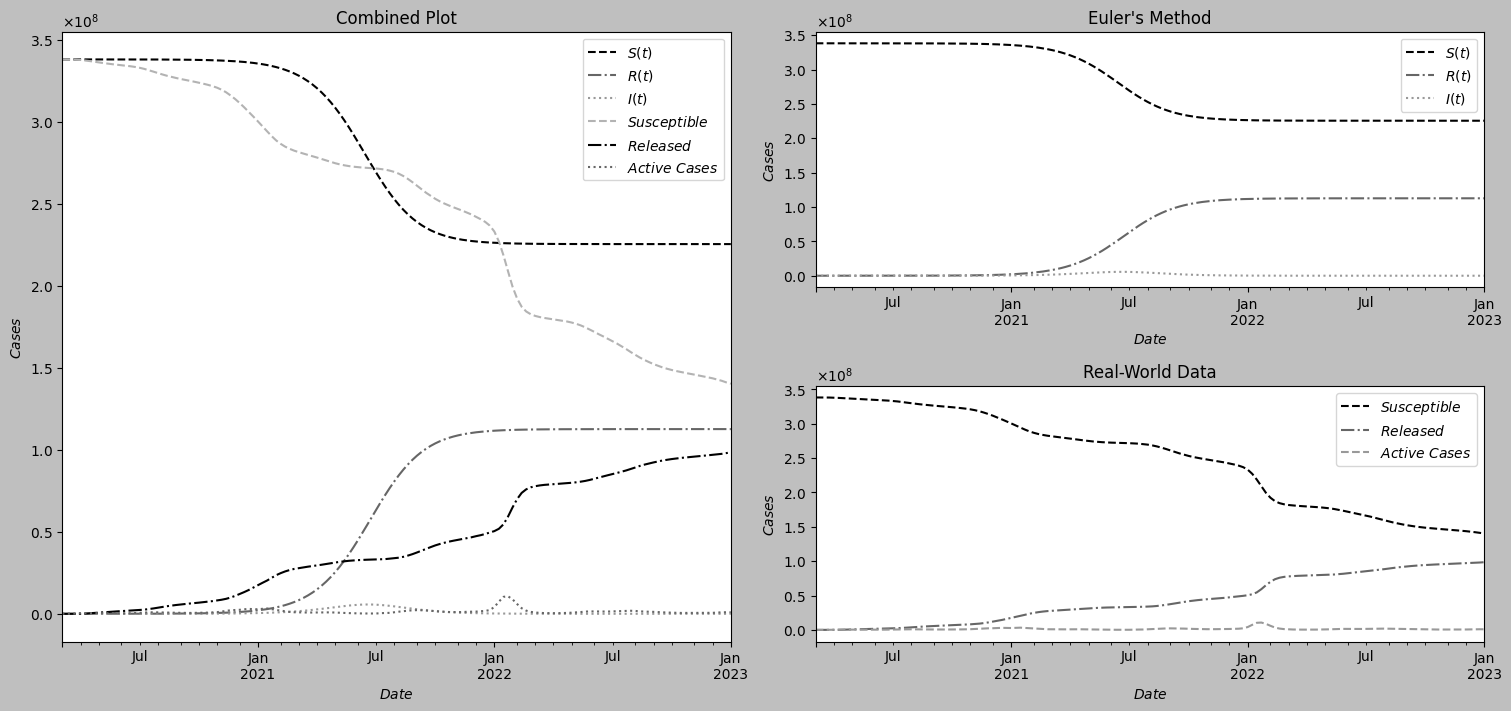
\includegraphics[width=16cm]{Figure_USAPredict.png}
\end{figure}
\begin{figure}[H]
	\caption{ARM Data}
	\centering
	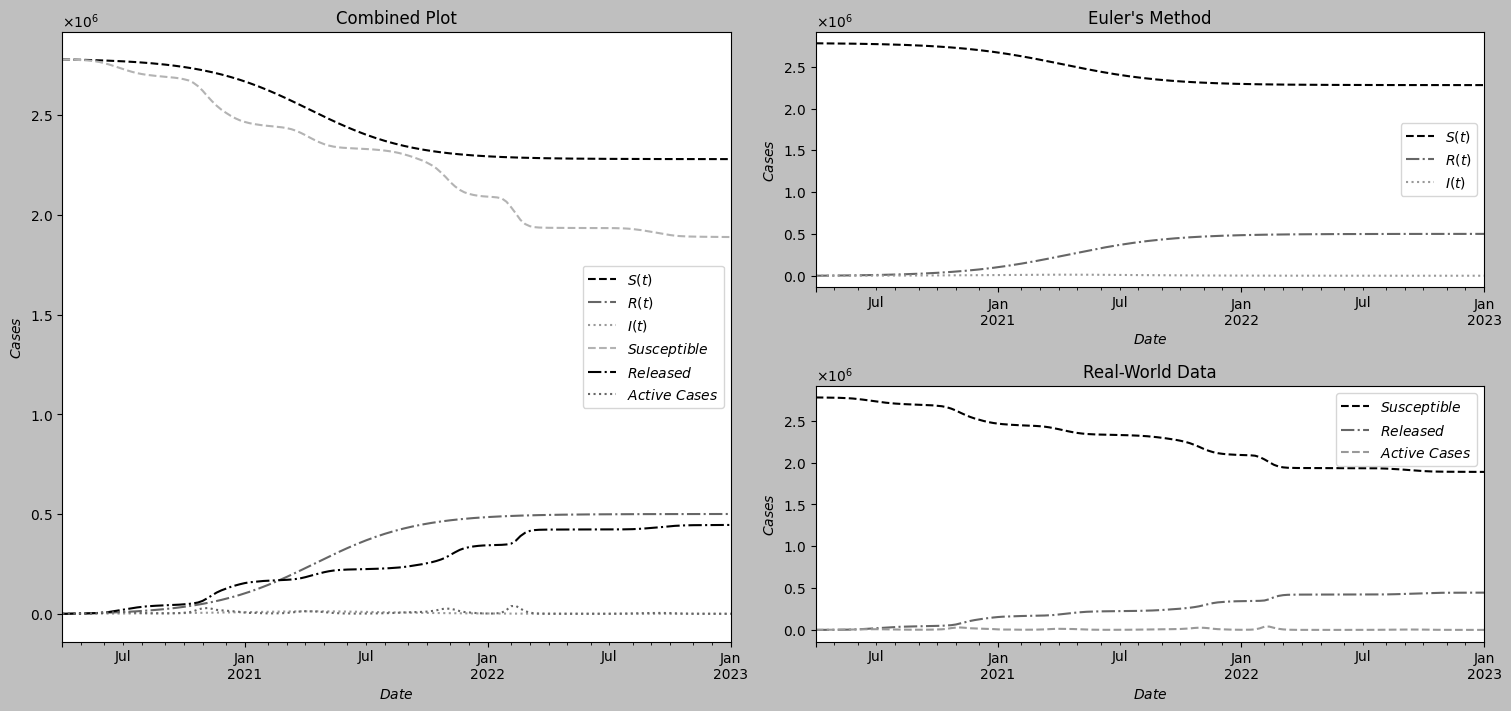
\includegraphics[width=16cm]{Figure_ArmPredict.png}
\end{figure}

\pagebreak

\subsection{Calculation \& RealWorld Use}\label{Applicaltions}
In both figures is depicted the prediction we obtained by using half the data 
of the Covid cases in their respective countries. The difficulty of predictions stems from
trying to correctly identify the optimal values for $\alpha$ and $\beta$. Firstly we need to defined what we mean 
by "optimal" values. In this case optimal was defined in a way such that the function

\begin{equation*}
	\sum_{t=0}^{n} (y(t)-y_t)^2 
\end{equation*}

is minimal. \\

Here $y(t)$ is the real world data of susceptible, infected or recovered data in time $t$. 
And $y_t$ is the point in the same time $t$ that we obtained by approximating the data with the SIR model.
Hence we want values of $\alpha$ and $\beta$ such that

\begin{equation*}
	\sum_{t=0}^{n} (S(t)-S_t)^2 + \sum_{t=0}^{n} (I(t)-I_t)^2 + \sum_{t=0}^{n} (R(t)-R_t)^2
\end{equation*}

is minimal.\\

Calculating this function for $\alpha$ and $\beta$ is a very difficult task and even the 
approximations we provided are not optimal, so we went with the brute force approach.\\
We took half the data and calculated the points for the Euler's approximation with different values for 
$\alpha$ and $\beta$. Lastly we calculated the error for each combination of $\alpha$ and $\beta$ and took 
the ones corresponding to the min of the error. What we obtained were not the most optimal values but they were still 
close. 

In Figure 2 and 3 we can see that the SIR model can to some extent predict the progression of the disease, but since the 
real world data is complex and involves a lot of other factors, it is not ideal. Those factors can include the lockdown, social distancing,
vaccines and a lot more. Hence fully predicting the progression of the diseases will not be possible, but we can still infer some useful information,
such as when approximately the diseases will plateau and what development can we expect from it in general. 
\section{Conclusion}\label{Conclusion}\thispagestyle{SectionFirstPage} % Hide headers on the first page of the section
\hspace{\parindent} In conclusion, our exploration of the SIR model, both
analytically and numerically, has provided valuable insights
into its dynamics and applications, particularly in the context
of understanding and combating pandemics at the early stage and predicting the spread
 and the numbers of infected, susceptible, and recovered quarters over time, hence
being ready to make the necessary decision of precautionary processes.
\par Through solving the SIR system of ordinary differential equations analytically, and
then numerically, we were able to compare the possible outcome given the parameters and initial values,
 and check if the SIR model gives a dependable source to rely on the pandemic clinical research.
According to the graphs we obtained through comparing the Euler's method, backward Euler's method, and the Analytical solution
given the necessary initial data, we obtained almost identical results and decided to apply one of the methods to the real data
to see if it is possible to get a small error with the real data on COVID-19.
\par The tests came in successful, and even though there are still errors present between the
approximation and the real data, we can confidently say, that using the model with
one of the given methods in the early stage of pandemics will give us insights into how big of a threat
the disease is and how concerned should the researchers be, hence getting a more precise insight on
the regulations of the precautionary behavior for the whole population.
\par Thus the practical relevance of the SIR model in informing public health policies
and interventions were proved as well. By accurately capturing the dynamics of disease transmission
and the impact of control measures, the SIR model can aid policymakers in making
informed decisions to mitigate the spread of infectious diseases and minimize their societal impact.
\par Looking ahead, our study underscores the importance of continued research into mathematical
models like the SIR model, not only for understanding current pandemics like COVID-19 but also
for preparedness against future infectious disease outbreaks. By refining and extending these
models, incorporating additional complexities and real-world data, we can enhance our ability
to forecast epidemic trends, evaluate intervention strategies, and ultimately safeguard public
health on a global scale.



% Appendices, remove if unused
\appendix
\renewcommand\thefigure{\thesection.\arabic{figure}}
\renewcommand\thetable{\thesection.\arabic{table}} % Renew figure and table counters and have the appendix letter before it
\lhead{\nouppercase{\rightmark}} % Renew headers
\rhead{}
\section{Appendix: Extensions and Modifications}\label{appendix-a}\thispagestyle{SectionFirstPage} % Hide headers on the first page of the section
\setcounter{figure}{0}
\setcounter{table}{0}
\lhead{Extensions and Modifications}
\hspace{\parindent}The basic SIR model can be expanded and modified in various ways to incorporate factors such as death and birth rates, vaccination rates, reinfection rates, and other significant variables, leading to more accurate calculations and predictions.
One famous modification was made by Yamamoto \cite{Satoru_Yamamoto}.
Let death rate be denoted by $\alpha$ and death rate be denoted by $\mu$.
The birth rate contributes to an increase in the size of the susceptible population, while the death rate leads to a decrease in its size.
The extent of this change can be calculated as:
\begin{equation*}
    \frac{\partial s}{\partial t} = \alpha - \mu s(t) - \beta s(t)i(t)
\end{equation*}
\hspace{\parindent}Yamamoto made another modification of the SIR model.
In this modification he took into consideration the inoculation rate of vaccine.
Let $\varepsilon$ be the rate at which individuals are vaccinated within a given population.
Incorporating this parameter leads to an increase in the population within the recovered group, thus resulting in the following modifications to the model equations:
\begin{equation*}
    \frac{\partial s}{\partial t} = \alpha(1 - \varepsilon) - \mu s(t)i(t)
\end{equation*}
\begin{equation*}
    \frac{\partial i}{\partial t} = \beta s(t)i(t) - (\gamma + \mu)(t)
\end{equation*}
\begin{equation*}
    \frac{\partial r}{\partial t} = \alpha\varepsilon + \gamma i(t) - \mu r(t)
\end{equation*}
\hspace{\parindent}Satoru Yamamoto examined the combined impact of both vaccination and the rate of reinfection as well.
A small portion of the population might get reinfected at a reinfaction rate $\sigma$.
The equation will look in the following way after making the modification:
\begin{equation*}
    \frac{\partial s}{\partial t} = \alpha(1 - \varepsilon) - \mu s(t)i(t)
\end{equation*}
\begin{equation*}
    \frac{\partial i}{\partial t} = \beta[s(t) + \sigma r(t)]i(t) - (\gamma + \mu)(t)
\end{equation*}
\begin{equation*}
    \frac{\partial r}{\partial t} = \alpha \varepsilon + \gamma i(t) - \mu r(t) - \beta \sigma r(t)i(t)
\end{equation*}
\hspace{\parindent}There is an extension of the SIR model which gives more realistic result.
The model is called SEIR, where ``E'' stands for ``exposed''.
The intensity of the virus depends on the exposure of an individual to the symptomatic asymptomatic carrier of the virus.
According to Peter Turchin \cite{Peter_Turchin} there is a need to add another group of exposed individuals to have a more effective model.
That group stage would be between susceptible and infected stages.
It will represent a group of individuals who have encountered the infection but are currently not infected.
Let $e(t)$ be the fraction of the population which is exposed to infection but is not infected.
As it was obtained above, for the standard SIR model the rate of change for the susceptible group is:
\begin{equation*}
    \frac{\partial s}{\partial t} = -\beta s(t)  i(t)
\end{equation*}
Let $\delta$ be the coefficient which shows the possibility of an exposed person contracting the infection.
Then the rate of change of the exposed group can be calculated as:
\begin{equation*}
    \frac{\partial e}{\partial t} = \beta s(t)  i(t) - \delta e(t)
\end{equation*}
Since there is a possibility for exposed individuals to contract the infection, the influence of \textit{susceptibles} on the rate of infected persons is positive.
Additionally, considering the possibility for infected individuals to recover, the impact of \textit{recovery} on the rate of infected persons is negative.
Thus:
\begin{equation*}
    \frac{\partial i}{\partial t} = \delta e(t) - \gamma i(t)
\end{equation*}
Similarly, the rate of change of the recovered group is:
\begin{equation*}
    \frac{\partial r}{\partial t} = \gamma i(t)
\end{equation*}
Combining all the equations above will ge the following system of differential equations:
\[
\left\{
    \begin{array}{l}
        \frac{\partial s}{\partial t} = -\beta s(t)  i(t)\\
        \frac{\partial e}{\partial t} = \beta s(t)  i(t) - \delta e(t)\\
        \frac{\partial i}{\partial t} = \delta e(t) - \gamma i(t)\\
        \frac{\partial r}{\partial t} = \gamma i(t)
    \end{array}
\right.
\]

\section{Appendix B}\label{appendix-b}\thispagestyle{SectionFirstPage} % Hide headers on the first page of the section
\setcounter{figure}{0}
\setcounter{table}{0}
This is the Appendix B.


% Bibliography
\newpage
\thispagestyle{SectionFirstPage} % Hide headers on the first page of the section
\lhead{References}
\rhead{}
\renewcommand\refname{References}
\printbibliography
\end{document}
